\chapter{Fundamentos Técnicos}
\label{chap:fmtos-técnicos}


\lettrine{E}{n} este capítulo realizaremos una aproximación a las diferentes tecnologías usadas en el desarrollo del presente \acrshort{tfg}.


\section{Jakarta EE}
\label{sec:jakartaEE}


\acrlong{jee} es un conjunto de especificaciones que amplía \acrlong{jse} con especificaciones para características empresariales como pueden ser la informática distribuida y los servicios web.Las aplicaciones de \acrshort{jee} manejan transacciones, seguridad, escalabilidad, concurrencia y administración de los componentes que está implementando. Entre las áreas en las que se utiliza \acrshort{jee} se encuentran el comercio electrónico, la  contabilidad o los sistemas de información bancaria~\cite{WikiJakartaEE-engl}.

Jakarta EE ofrece a los desarrolladores un conjunto completo de especificaciones abiertas y neutrales para proveedores que se utilizan para desarrollar aplicaciones Java modernas y nativas de la nube desde cero. Ofrece una combinación de ventajas que no se pueden encontrar en otros marcos Java: Madurez, estabilidad y retrocompatibilidad. Su flexibilidad arquitectónica permite arquitecturas de microservicios basadas en la nube, así como arquitecturas tradicionales y monolíticas. Se rata de una plataforma con todas las funciones que se puede configurar en solo unas pocas docenas de líneas de código y con capacidad de cambiar fácilmente las tecnologías subyacentes para cumplir con los nuevos requisitos y aprovechar las implementaciones más rápidas y ligeras. Todo esto brinda a los desarrolladores y empresas de Java todo lo que necesitan para construir y evolucionar aplicaciones Java nativas de la nube hoy y en el futuro~\cite{JakartaEE-eclipse}.

\subsection{Historia}
\label{sec:historia}

El lenguaje de programación Java nació en 1991 de la mano de James Gosling, que en aquellos momentos trabajaba en Sun Microsystems, y su equipo. Los objetivos de Gosling eran implementar una máquina virtual y un lenguaje con una estructura y sintaxis similar a C++. La promesa inicial de Gosling era  \textquote{\textit{Write Once, Run Anywhere}} (Escríbelo una vez, ejecútalo en cualquier lugar), proporcionando un lenguaje independiente de la plataforma y un entorno de ejecución ligero y gratuito para las plataformas más populares (la \acrfull{jvm}), de forma que los binarios (bytecode) de las aplicaciones Java pudiesen ejecutarse en cualquier plataforma. En 1995 fue lanzado comercialmente por Sun Microsystems como un componente fundamental de la plataforma Java~\cite{WikiJava-esp}. 

La plataforma Java es un conjunto de programas que facilitan el desarrollo y la ejecución de programas escritos en el lenguaje de programación Java~\cite{WikiJavaSwPlatform}. Una plataforma Java incluye un motor de ejecución (la \acrshort{jvm}), un compilador y un conjunto de bibliotecas. También puede haber servidores adicionales y bibliotecas alternativas que dependen de los requisitos. Las plataformas Java se han implementado para una amplia variedad de hardware y sistemas operativos con el fin de permitir que los programas Java se ejecuten de manera idéntica en todos ellos. Existen distintas plataformas orientadas adistintas clases de dispositivos y aplicaciones, a saber:

\begin{itemize}
\item Java Card: Una tecnología que permite que las pequeñas aplicaciones basadas en Java (applets) se ejecuten de forma segura en tarjetas inteligentes y dispositivos similares de pequeña memoria. 
\item Java ME (Micro Edition): especifica varios conjuntos diferentes de bibliotecas (conocidas como perfiles) para dispositivos con capacidades limitadas de almacenamiento, visualización y energía. A menudo se utiliza para desarrollar aplicaciones para dispositivos móviles, PDA, decodificadores de TV e impresoras. 
\item Java SE (Standard Edition): Para uso general en PC de escritorio, servidores y dispositivos similares. 
\item Jakarta EE (Enterprise Edition): conjunto de Java SE junto a varias API que son útiles para aplicaciones empresariales cliente-servidor de varios niveles.
\end{itemize}


Puesto que el desarrollo de este trabajo ha sido a través de Jakarta EE, que nos centraremos en dicha plataforma. Java Enterprise Edition fue un proyecto iniciado por Sun Microsystems en el año 1999 bajo el nombre de J2EE y adquirida por Oracle diez años más tarde, dando continuidad al proyecto hasta 2017, momento en el que el proyecto pasó a manos de la Eclipse Foundation, quien continúa con su desarrollo bajo la modalidad de código abierto en la actualidad ~\cite{JakartaEE-eclipse}.

Esta transferencia de proyecto de Oracle a Eclipse Foundation no incluyó el uso de la marca Java, por lo que Eclipse Foundation renombró el proyecto pasando a denominarse Jakarta EE. La primera versión lanzada bajo el parguas de Eclipse Foundation fue la 8 (versión con la que se ha desarrollado la aplicación de este \acrshort{tfg}) y actualmente está disponible la versión 9.1 (página~\pageref{tab:evolucionJavaEE}).


\begin{table}[hp!]
  \centering
  \rowcolors{2}{white}{udcgray!25}
  \begin{tabular}{c|c|c|c}
  \rowcolor{udcpink!25}
  \textbf{Versión} & \textbf{Año} & \textbf{Soporte Java SE} & \textbf{Empresa} \\hline
J2EE 1.2 & 1999 & J2SE 1.2 & Sun Microsystems \\
J2EE 1.3 & 2001 & J2SE 1.3 & Sun Microsystems \\
J2EE 1.4 &2003 & J2SE 1.4 & Sun Microsystems \\
Java EE 5 & 2006 & Java SE 5 & Sun Microsystems \\
Java EE 6 & 2009 & Java SE 6 & Oracle \\
Java EE 7 & 2013 & Java SE 7 & Oracle \\
Java EE 8 & 2017 & Java SE 8 & Oracle \\
Jakarta EE 8 & 2019 & Java SE 8 & Eclipse Foundation \\
Jakarta EE 9 & 2020 & Java SE 8 & Eclipse Foundation \\
Jakarta EE 9.1 & 2021 & Java SE 11//Java SE 8 & Eclipse Foundation \\
  \end{tabular}
  \caption{Evolución de Java EE}
  \label{tab:evolucionJavaEE}
\end{table}



\subsection{Arquitectura Jakarta EE}
\label{sec:arquitectura}


\acrshort{jee} se define por su especificación. La especificación define las \acrfull{api} y sus interacciones. \acrshort{jee} incluye varias especificaciones que sirven para diferentes propósitos, como pueden ser generar páginas web, leer y escribir desde una base de datos de manera transaccional, administrar colas distribuidas. Las \acrshort{api} de \acrshort{jee} incluyen varias tecnologías que amplían la funcionalidad de las \acrshort{api} de Java SE base, como Jakarta Enterprise Beans, conectores, servlets, Jakarta Server Pages y varias tecnologías de servicios web~\cite{WikiJakartaEE-engl}. En la figura ~\ref{fig:arquitecturaJakartaEE} se muestra la arquitectura \acrshort{jee} (página ~\pageref{fig:arquitecturaJakartaEE})\cite{WikiJakartaEE-engl}.


\begin{figure}[hp!]
  \centering
  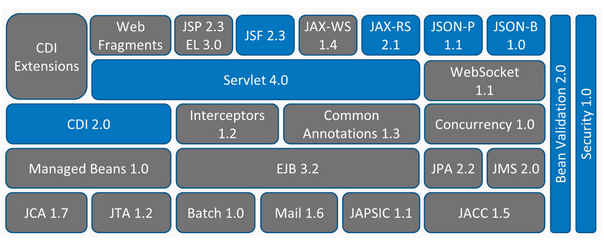
\includegraphics[width=0.50\textwidth]{imaxes/JakartaEE-Architecture.png}
  \caption{Arquitectura Jakarta EE}
  \label{fig:arquitecturaJakartaEE}
\end{figure}

Entre las distintas especificaciones de \acrshort{jee} cabe destacar las siguientes:

\begin{itemize}
   \item Especificaciones web
     \begin{itemize}
       \item Jakarta Servlet: define cómo gestionar las solicitudes \acrfull{http}, de forma síncrona o asíncrona. Es de bajo nivel y otras especificaciones de \acrshort{jee} dependen de él.
	   \item Jakarta WebSocket: define un conjunto de \acrshort{api} para dar servicio a las conexiones de WebSocket
   	   \item \acrlong{jsf}: una tecnología para construir interfaces de usuario a partir de componentes.
  	   \item Jakarta \acrlong{el} es un lenguaje simple diseñado originalmente para satisfacer las necesidades específicas de los desarrolladores de aplicaciones web.
     \end{itemize} 
   \item Especificaciones de servicios web
     \begin{itemize}
       \item Jakarta RESTful Web Services: proporciona soporte en la creación de servicios web de acuerdo con el patrón arquitectónico de \acrfull{rest}.
  	   \item Jakarta JSON Processing: conjunto de especificaciones para gestionar la información codificada en formato \acrfull{json}.
	   \item Jakarta JSON Binding: proporciona especificaciones para convertir información \acrshort{json}. en o desde clases Java
 	   \item Jakarta XML Binding: permite asignar \acrfull{xml} a objetos Java; Los servicios Web \acrshort{xml} de Jakarta se pueden utilizar para crear servicios web \acrfull{soap}.
     \end{itemize}
   \item Especificaciones empresariales
     \begin{itemize}
        \item Jakarta Activation (JAF): especifica una arquitectura para extender los beans de componentes proporcionando tipos de datos y enlaces de dichos tipos. 
        \item Jakarta \acrfull{cdi}: es una especificación para proporcionar un contenedor de inyección de dependencias
        \item \acrfull{ejb} define un conjunto de \acrshort{api} ligeras que un contenedor de objetos (el contenedor \acrshort{ejb}) admitirá para proporcionar transacciones, llamadas a procedimientos remotos, control de simultaneidad, inyección de dependencias y control de acceso para objetos de negocio. Este paquete contiene las clases e interfaces de \acrshort{ejb} que definen los contratos entre el bean empresarial y sus clientes y entre el bean empresarial y el contenedor ejb. 
        \item \acrfull{jpa}: especificaciones sobre el mapeo objeto-relacional entre tablas de bases de datos de relaciones y clases Java.
        \item \acrfull{jta}: contiene las interfaces y anotaciones para interactuar con el soporte de transacciones ofrecido por Jakarta EE.
	    \item \acrfull{jms} proporciona una forma común para que los programas Java creen, envíen, reciban y lean los mensajes de un sistema de mensajería empresarial.      
     \end{itemize}
   \item Otras especificaciones
     \begin{itemize}
        \item Validación: contiene las anotaciones e interfaces para el soporte de validación declarativa ofrecido por la \acrshort{api} de validación de Bean. 
		\item Jakarta Batch: proporciona los medios para que el procesamiento por lotes en aplicaciones ejecute tareas en segundo plano de larga duración que posiblemente impliquen un gran volumen de datos y que puedan necesitar ser ejecutadas periódicamente. 
		\item Jakarta Connectors: herramienta basada en Java para conectar servidores de aplicaciones y \acrfull{eis} como parte de la integración de \acrshort{eai}. Esta es una \acrshort{api} de bajo nivel dirigida a proveedores con los que el desarrollador de aplicaciones promedio generalmente no entra en contacto.
     \end{itemize}
\end{itemize}




\subsection{Componentes Jakarta EE}
\label{sec:componentes}
\acrshort{jee} define cuatro tipos de componentes de aplicación~\cite{jee}: 

\begin{itemize}
   \item Aplicaciones cliente: suelen ser programas \acrfull{gui} que se ejecutan en un equipo de escritorio.
   \item Applets: son componentes de \acrshort{gui} que normalmente se ejecutan en un navegador web, pero pueden ejecutarse en una variedad de otras aplicaciones o dispositivos que admiten el modelo de programación de applets. 
   \item Aplicaciones web como servlets, páginas \acrfull{jsp} y \acrshort{jsf} que se ejecutan en un contenedor web y responden a las peticiones \acrshort{http} del cliente.
   \item Aplicaciones empresariales como los componentes \acrshort{ejb}, \acrshort{jta} o \acrshort{jms}, que se ejecutan en un contenedor \acrshort{ejb} .
\end{itemize}



\subsection{Contenedores}
\label{sec:contenedores}
\acrshort{jee} se divide en dominios lógicos llamados contenedores. En una aplicacion \acrshort{jee} los componentes nunca interactúan con otros componentes de la aplicación si no que utilizan los protocolos y métodos del contenedor para interactuar entre sí y con los servicios de la plataforma~\cite{JakartaEE}. Cada contenedor tiene una función específica, soporta un conjunto de \acrshort{api} y ofrece servicios a los componentes tales como seguridad, acceso a base de datos, gestión de transacciones, nombres de directorios e inyección de recursos. Los contenedores ocultan la complejidad técnica y mejoran la portabilidad lo que permite al desarrollador centrarse en la lógica de aplicación en lugar de resolver problemas técnicos. Por ejemplo el contenedor \acrshort{ejb} es responsable de administrar la ejecución de los beans que contienen la lógica de negocio.

\subsubsection{Servidores}
\label{sec:servidores}
Detrás de un contenedor \acrshort{jee} se encuentra el servidor del que forma parte~\cite{JakartaEE}. Un proveedor de productos de \acrshort{jee}  por lo general implementa la funcionalidad del lado del servidor de \acrshort{jee}  usando una infraestructura de transacciones existente en combinación con la tecnología \acrshort{jse} de la plataforma Java. La funcionalidad del cliente \acrshort{jee} se basa por lo general en la tecnología \acrshort{jse} .




\section{Librerías y componentes Jakarta EE usados}
\label{sec:componentesJakartaEE}

A continuación ofrecemos una relación de las principales librerías y componentes \acrshort{jee} usados en el desarrollo de este \acrshort{tfg}.

\subsection{Jakarta Enterprise Bean}
\label{sec:jeb}

Un \acrfull{ejb} es un componente del lado del servidor que encapsula la lógica empresarial de una aplicación. La lógica de negocio es el código que cumple el propósito de la aplicación~\cite{JEE7-Tutorial}.

Estos componentes se ejecutan en el contenedor \acrshort{ejb}. Aunque es transparente para el desarrollador de aplicaciones, el contenedor \acrshort{ejb} proporciona servicios a nivel de sistema tales como transacciones y seguridad a sus enterprise beans. Estos servicios le permiten crear e implementar rápidamente \acrshort{ejb}, que son los que forman el núcleo de las aplicaciones transaccionales de \acrshort{jee}.

Entre las ventajas que ofrecen los \textit{enterprise beans} se encuentran los siguientes:
\begin{itemize}
\item Simplifican el desarrollo de la aplicación ya que es el contenedor \acrshort{ejb} el que se encarga de gestionar los servicios a nivel de sistema, como la gestión de transacciones y la autorización de seguridad.
\item La lógica del negocio reside en los \textit{enterprise beans} y no en el lado del cliente, permitiendo que el desarrollo del lado del cliente este desacoplado de la lógica del negocio.
\item Los \textit{enterprise beans} son componentes portables, reutilizables y pueden ser desplegados en servidores que usen los estándares del  \acrshort{jee} \acrshort{jee}.
\item Pueden residir en diferentes servidores pudiendo ser invocados por un cliente remoto.
\end{itemize}

El uso \textit{enterprise beans} está recomendado en aplicaciones escalables, en aquellas en las que necesitemos asegurar la integridad de los datos y/o en aplicaciones con variedad de clientes.


\subsection{Java Server Faces}
\label{sec:jsf}
\acrfull{jsf} es una tecnología para el desarrollo de \acrshort{gui} en aplicaciones web dentro de la plataforma \acrshort{jee}~\cite{DesarrolloJakartaEE}.

La especificación está definida por \acrfull{jcp}, lo que lo convierte en un estándar. Se basa en la utilización del patrón  \acrfull{mvc} que tiene como objetivo separar los datos (modelo) de su procesamiento (controlador) y la forma en la que estos son presentados al usuario en una aplicación (vista).\acrshort{jsf} oculta al programador los detalles de las peticiones y respuestas \acrshort{http}, simplificando la programación de aplicaciones web y acercándolas a un estilo de desarrollo similar al de las aplicaciones de escritorio.

En \acrshort{jsf} se define un servlet llamado Faces Servlet dentro de un archivo de configuración llamado \textit{web.xml}, que tiene como objetivo recibir las distintas solicitudes \acrshort{http} de los cliente y procesarlas. 

\subsubsection{Ciclo de vida de una aplicación JSF}
\label{sec:ciclo-vida-jsf}
El ciclo de vida de una aplicación \acrshort{jsf} consta de las siguientes fases~\cite{DesarrolloJakartaEE}:

\begin{enumerate}
\item Restaurar la vista: en esta etapa \acrshort{jsf} comprueba si la solicitud \acrshort{http} recibida es nueva o no con el fin de crear o restaurar el árbol de componentes (objetos Java necesarios).
\item Aplicar los valores de la solicitud: una vez creado el arbol cada componente actualiza sus valores con los parámetros presentes en la solicitud.
\item Procesar validaciones: Valida y convierte los datos que el usuario ingresó al tipo que corresponda. En caso de que se produzca algún error, se saltará a la etapa de renderización, en la que se le informará al usuario de los errores producidos. En caso contrario se pasará a la siguiente fase (actualizar valores).
\item Actualizar los valores del modelo: se refresca el árbol de componentes actualizando los valores del modelo.
\item Invocar la lógica de la aplicación: se invocan los métodos solicitados por el usuario.
\item Renderizar la respuesta: se envía al cliente la respuesta en \acrshort{html}.
\end{enumerate}


\subsection{Primefaces}
\label{sec:primefaces}

Primefaces es una librería de componentes visuales open source que cuenta con un amplio conjunto de componentes enriquecidos para diseñar interfaces de usuario creada por PrimeTek Informatics. El desarrollo inicial de PrimeFaces se inició a finales de 2008\cite{WikiPrimefaces}.

Las principales características que presenta son las siguientes~\cite{Primefaces}:

\begin{itemize}
\item Amplio conjunto de componentes (HtmlEditor, Dialog, Autocompletar, Gráficos y muchos más).
\item Soporte nativo AJAX basado en API JSF AJAX estándar. 
\item Ligero, sin necesidad de dependencias ni configuraciones adicionales. 
\item Capacidad de respuesta y accesibilidad incorporadas. 
\item Amplia documentación y comunidad de usuarios.
\end{itemize}


\subsection{Omnifaces}
\label{sec:omnifaces}

OmniFaces es una biblioteca de utilidades open source para \acrshort{jsf} desarrollada por dos miembros de la JSF Expert Group (JSF EG), Bauke Scholtz (alias BalusC) y Arjan Tijms\cite{WikiOmnifaces}.

A diferencia de otras bibliotecas de componentes \acrshort{jsf}  existentes en el mercado (como PrimeFaces, BootsFaces o ButterFaces), OmniFaces no contiene ningún componente orientado a enbellecer la visualización, si no que está más orientado a las "utilidades" que resuelven problemas prácticos cotidianos y soluciones para (pequeñas) deficiencias en la \acrshort{api}  \acrshort{jsf}. Esta librería se centra en utilidades que facilitan las tareas cotidianas con la \acrshort{api} \acrshort{jsf} estándar. Estamos ante una respuesta a los problemas recurrentes con los que los autores se han encontrado a lo largo de su desarrollo profesional con \acrshort{jsf} y de las preguntas que se publican en Stack Overflow.

\subsection{Java Object Oriented Querying}
\label{sec:jooq}
\acrfull{jooq} es una biblioteca de software de asignación de bases de datos ligera en Java que implementa el patrón de registro activo desarrollada por Lukas Eder. Su propósito es ser tanto relacional como orientado a objetos al proporcionar por un lado un lenguaje específico del dominio para construir consultas SQL seguras y por otro generar clases a partir de un esquema de base de datos a través de su \acrshort{api} fluida sobre las que construir dichas consultas.~\cite{jooqBaeldung, WikiJooq}.

El enfoque de \acrshort{jooq} pone el foco en el lado de \acrfull{sql} en lugar de \acrshort{jpa} como hacen los \acrfull{orm} como por ejemplo Hibernate.

Alguna de las características que presenta \acrshort{jooq} son las siguientes\citep{VentajasJooq}:


\begin{itemize}
\item Proporciona un generador de código que permite, mediante ingeniería inversa, converir el esquema de base de datos en conjunto de tablas de modelado de clases Java, registros, secuencias, POJO, DAO, procedimientos almacenados, tipos definidos por el usuario y muchos más listas para usarse. 
\item Ofrece la posibilidad de utilizar toda la funcionalidad de la base de datos seleccionada en lugar de una abstracción o un subconjunto limitado gracias a su \acrfull{dsl} fluido que se asigna uno a uno con \acrshort{sql}
\item El \acrfull{dsl} que genera permite que su IDE se complete automáticamente mientras escribe las consultas.
\item Utiliza el sistema de tipos de Java para garantizar que el SQL que genera es válido.
\item La \acrshort{api} de \acrshort{jooq} hace todo lo posible para asegurarse de que está utilizando el tipo de datos Java correcto para cada columna de su base de datos. 
\item Presenta una extensión de conversor de tipos fácil de usar para transformar tipos de datos comunes, como Timestamp o \acrshort{sql} Date/Time a java.time.ZonedDateTime.
\item Existe una funcionalidad de mapeo que ayuda a asignar conjuntos de resultados a \acrfull{pojo} y proporciona una implementación del patrón de registro activo para trabajar de una manera similar a \acrshort{orm}
\item Se pueden usar los streams existentes a partir de Java 8 para transformar conjuntos de resultados de forma fácil y sucinta.
\item Si se producen cambios en el esquema de la base de datos se obtienen errores de compilación en lugar de los de tiempo de ejecución.
\item Funciona con las principales bases de datos relacionales: MS Access, MS Access 2013, CUBRID, IBM DB2, Apache Derby, Firebird, H2, Hypersonic, Informix, Ingres, MariaDB, MySQL, Oracle, Oracle, PostgreSQL, SQLite, SQL Server, SQL Server y Sybase.
\item Tiene doble licencia, siendo de uso gratuito para todas las bases de datos de código abierto.
\end{itemize}

\subsection{Log4j}
 Es una biblioteca \gls{opensource} perteneciente a los Java Logging Frameworks desarrollada en Java por la Apache Software Foundation que permite generar mensajes de logging de una forma limpia, sencilla, permitiendo filtrarlos por importancia y pudiendo configurar su salida por vía consola, fichero u otras distintas.
 
  Existen diversos niveles de prioridad. A continuación se muestran los más utlizados
  
\begin{itemize}
\item DEBUG: usado para escribir mensajes de depuración.
\item INFO: mensajes puramente informativos.
\item WARN: alertas. Generealmente utilizados para alertar de eventos de los que se quiere dejar constancia pero que no afectan al correcto funcionamiento de la aplicación.
\item ERROR: usado para mensajes de eventos que afectan al programa pero lo dejan seguir funcionando (por ejemplo un parámetro figura como vacío por lo que se se carga el parámetro por defecto).
\item FATAL: usado para errores críticos. 
\end{itemize}  
  
    


\section{Formatos de almacenamiento. PostgreSQL}
\label{sec:almacenamiento}

Los datos se han almacenado en una base de datos relacional. Para ello se ha optado por el gestor de base de datos de código abierto PostgreSQL, ya que es una solución robusta, con amplias funcionalidades, con un uso cada vez más extendido y es 100\% open source~\cite{PostgreSQL}.



\subsection{Historia}
\label{sec:historiapsql}

El sistema de gestión de bases de datos objeto-relacionales ahora conocido como PostgreSQL se deriva del paquete POSTGRES escrito en la Universidad de California en Berkeley. Con más de dos décadas de desarrollo a sus espaldas, PostgreSQL es ahora la base de datos de código abierto más avanzada disponible en cualquier lugar.

\subsubsection{Inicios. POSTGRES}
\label{sec:postgres}

La implementación de POSTGRES comenzó en 1986. Desde entonces ha tenido varios lanzamientos importantes. El primer sistema "demoware\footnote{Tipo de software que permite su uso sin ninguna restricción por un período limitado de tiempo, por un número de usos o por progresión hasta un determinado punto. Generalmente pasado el período de prueba, se deshabilitan todas las funciones o parte de ellas.} " entró en funcionamiento en 1987 y se mostró en la Conferencia ACM-SIGMOD de 1988. La versión 1 fue lanzada a algunos usuarios externos en junio de 1989. La Versión 2 fue lanzada en junio de 1990 con un nuevo sistema de reglas. La versión 3 apareció en 1991 y agregó soporte para múltiples administradores de almacenamiento, un ejecutor de consultas mejorado y un sistema de reglas reescrito. En su mayor parte, las versiones posteriores hasta Postgres95 se centraron en la portabilidad y la confiabilidad.

POSTGRES se ha utilizado para implementar muchas aplicaciones diferentes de investigación y producción. También se ha utilizado como una herramienta educativa en varias universidades. A finales de 1992, POSTGRES se convirtió en el principal gestor de datos del proyecto de computación científica Sequoia 2000.

\subsubsection{Postgres95}
\label{sec:postgres95}

En 1994, Andrew Yu y Jolly Chen agregaron un intérprete de lenguaje \acrshort{sql} a POSTGRES. Bajo un nuevo nombre, Postgres95 fue posteriormente lanzado a la web para encontrar su propio camino en el mundo como un descendiente de código abierto del código original de POSTGRES Berkeley. Estaba codificado completamente en ANSI C y redujo su tamaño un 25\% respecto al código original. También se mejoró el rendimiento y la capacidad de mantenimiento.

\subsubsection{PostgreSQL}
\label{sec:postgresql}

En 1996 se eligió un nuevo nombre, PostgreSQL, para reflejar la relación entre el POSTGRES original y las versiones más recientes con capacidad \acrshort{sql}. Al mismo tiempo se configuró la numeración de la versión para que comenzara en 6.0, poniendo los números de nuevo en la secuencia originalmente iniciada por el proyecto POSTGRES de Berkeley.

Durante el desarrollo de PostgreSQL el foco se trasladó hacia el aumento de las características y capacidades 

\subsection{Características}
\label{sec:caracteristicas}

PostgreSQL es compatible con una gran parte del estándar SQL y entre sus caraterísticas figuran las siguientes: 
\begin{itemize}
\item Es \textit{open source}
\item Emplea un lenguaje SQL estandar.lo que permite la importación de otras bases de datos.
\item Cumple con el modelo ACID (atomicidad, consistencia, aislamiento y durabilidad de los datos almacenados).
\item Capacidad de realizar consultas complejas.
\item Claves foráneas.
\item Triggers(disparadores).
\item Vistas actualizables.
\item Integridad transaccional.
\item Control de versiones simultánea.
\end{itemize}

También permite ampliaciones por parte del usuario de múliples formas, por ejemplo mediante la agregación de:
\begin{itemize}
\item Nuevos tipos de datos 
\item Funciones 
\item Operadores 
\item Funciones agregadas 
\item Lenguajes procedurales 
\item Extensiones
\end{itemize}


